\chapter{Related Work}\label{chapter:related_work}

In the following sections, we introduce benchmark frameworks that are designed to investigate the performance of RDF databases. In Section \ref{sec:benchmark_conclusions}, we summarize the frameworks and compare them to our work which is the introduction of a new approach to existing benchmark frameworks.

\section{Berlin SPARQL Benchmark}

\paragraph{Domain}
The Berlin SPARQL Benchmark (BSBM)~\cite{berlin} features an e-commerce use case in which a set of products is offered by different vendors and consumers who posted reviews about the products. 

\paragraph{Workload}
BSBM measures the SPARQL query performance of RDF-based tools via realistic workloads of queries based on the use cases. The benchmark defines three different use cases and a suite of benchmark queries---a \textit{mix} of queries---in each of them~\cite{berlin_specification}, simulating the search and navigation pattern of a consumer looking for a product. The queries include read and update operations as well.

\paragraph{Models}
BSBM generates artificial models in different sizes, by using normal distributions among the elements. For example, the number of reviews and different properties per product are distributed following a normal distribution.

\paragraph{Metrics}
The benchmark defines certain performance metrics that relate to the query execution times from different perspectives. The most important metrics are the following:
\begin{itemize}
	\item{\textit{Queries per Second}}: the number of queries executed within a second.
	\item{\textit{Query Mixes per Hour}}: the number of mixed queries with different parameters that evaluated within an hour.
	\item{\textit{Overall Runtime}}: the overall time that a certain amount of query mix requires.
\end{itemize}


\section{DBpedia SPARQL Benchmark}
The DBpedia SPARQL Benchmark (DBPSB) proposes a benchmark framework for RDF databases based on the DBpedia~\cite{dbpedia_data} knowledge base. It measures the performance of real queries that were issued against existing RDF data~\cite{dbpedia}. DBPSB generates models in various sizes trying to obtain a similar characteristic belonging to the original DBpedia dataset.\\
Similarly to BSBM, DBPSB also defines metrics to investigate the performance from different aspects, such as the \textit{Query Mixes per Hour} and \textit{Queries per Second}. 

\section{SP$^2$Bench}

The SPARQL Performance Benchmark (SP$^2$Bench)~\cite{sp2bench} is based on the \textit{Digital Bibliography and Library Project} (commonly known as \textit{dblp}) which provides an open bibliographic information on major computer science publications~\cite{dblp}. The benchmark queries are not explicitly evaluated over the \textit{dblp} dataset, since SP$^2$Bench uses arbitrarily large, artificially generated models for the measurements that are created to follow the characteristics of the original \textit{dblp} dataset, such as the power-law distribution.

SP$^2$Bench is designed to test the most common SPARQL constructs, operator constellations and a broad range of RDF data access patterns. Instead of defining a sequence of use case motivated queries, the framework proposes various systematic queries that cover specific RDF data management approaches.

Similarly to BSBM, SP$^2$Bench also measures additional performance related metrics besides the evaluation time, such as the disk storage cost, memory consumption, data loading time and success rates, hence, every metric captures different aspects from the evaluations.

\section{Train Benchmark Framework}\label{sec:train}

\subsection{Overview}

The Train Benchmark framework was designed and implemented by the Fault Tolerant Systems Research Group in the Budapest University of Technology and Economics~\cite{tb_report}. The benchmark investigates the performance of model validations via different graph queries by measuring the evaluation times of different RDF, SQL, EMF and graph databases.

An overview of the Train Benchmark framework is shown in Figure \ref{fig:overview_train}, illustrating the framework how connects the model validations to the database systems. In step 1, the framework generates a graph-based model derived from a particular domain. After defining different constraints (rules) on the domain---such as the presence of an edge between two types of nodes---the benchmark injects erroneous elements into the model (step 2.), which elements are considered as violations of the constraints. During step 3, the framework loads the invalid model to the particular database system.\\
Every constraint has a corresponding validation pattern that is the negation of the constraint and it includes a pattern of elements that violates the certain constraint (4.). Every validation pattern is defined in the query language of the particular database (5). Step 6 denotes the query evaluation that represents the model validation. The result set of the evaluation contains the invalid elements which violated the constraint. The performance indicator of the databases is the required time of model validation, so the query evaluation time.\\
Besides the validations, the framework also performs model transformations to alter the amount of invalid elements in the model. Every transformation is followed by another validation.

\begin{figure}[!ht]
	\centering
	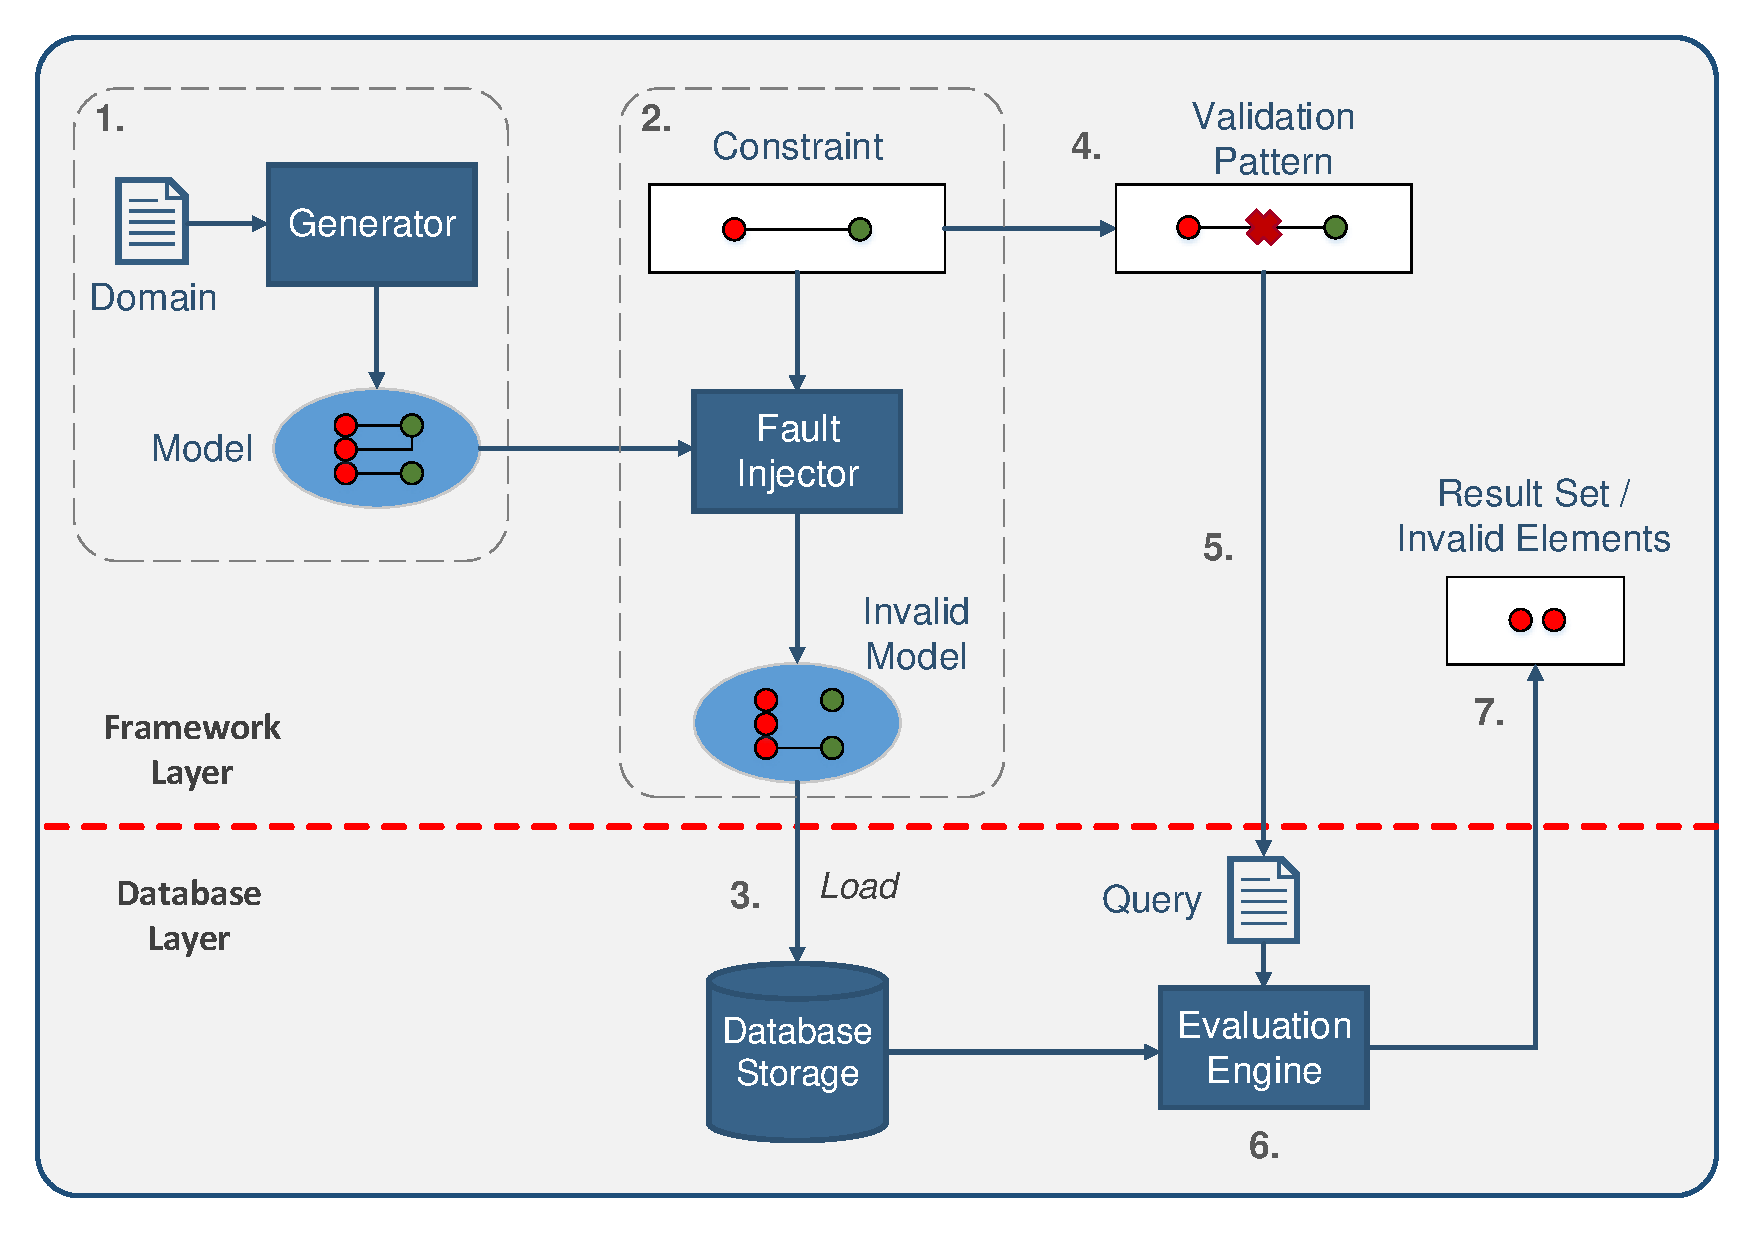
\includegraphics[width=150mm, keepaspectratio]{figures/functionality.pdf}
	\caption{An overview of Train Benchmark.}
	\label{fig:overview_train}
\end{figure}

\begin{figure}[!ht]
	\centering
	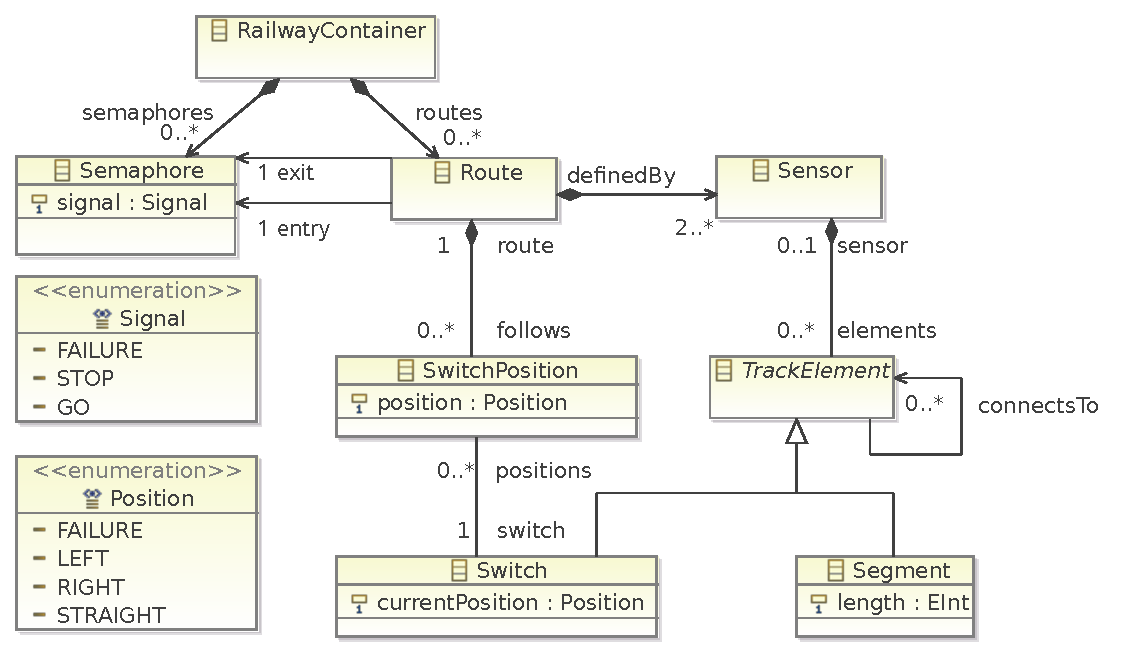
\includegraphics[width=150mm, keepaspectratio]{figures/railway-containments.pdf}
	\caption{The Railway domain of Train Benchmark.}
	\label{fig:tb_domain}
\end{figure}

\subsection{Model Generation}

The Train Benchmark framework uses artificially generated graph-based models for the measurements over a \textit{railway} domain, illustrated in Figure \ref{fig:tb_domain}. In the models, a train route is defined by a sequence of sensors, and the sensors are associated with track elements which are either segments or switches. A route follows certain switch positions which describe the required state of a switch belonging to the route. Each route has a semaphore on its entry and exit~\cite{train_ttc}.

The generated models over the Railway domain are not related to a real-life model, which leads to the fact that the cardinalities of the elements and their distributions do not follow a real model's characteristic, therefore, the measurement results of different databases cannot be claimed to be representative in a real-life use case.

\subsection{Metric-Based Analysis}

The Train Benchmark framework was extended with metric-based analysis in ~\cite{metric_ase}.


\section{Conclusion} \label{sec:benchmark_conclusions}

The represented benchmark frameworks propose different comprehensive use cases to assess the performance of graph queries typically over RDF data. BSBM and DBpedia use representative queries for the measurements that demonstrate real-life use cases, and the SP$^2$Bench framework concentrates on the creation of various systematic queries that investigate the specific RDF data management approaches. The Train Benchmark framework aims a different aspect of performance by concentrating on model validations via graph queries. As a conclusion, these frameworks guarantee a comprehensive performance evaluation of a workload---the model, query and tool---by emphasizing the impact of \textit{queries} to the performance.

However, in case of an arbitrary workload, the \textit{model} also represents a dominating factor to the performance. DBpedia or the SP$^2$Bench framework do not consider model modifications in their workloads, so they do not investigate the impact of various model characteristics to the performance, they only generate the same structural model in different sizes to measure scalability. BSBM proposes update operations on the models, still, it does not investigate model and performance correlations. Even though Train Benchmark considers model transformations, yet, it modifies only one type of element that impacts the result set of the query evaluation, and the generated models are still considered as static models. As a conclusion, all of the introduced frameworks concentrate on the generation of one static model without altering its internal structure and analyzing their influence to the performance.

In order to introduce a new approach to the field of graph-based benchmark frameworks, we focus on elaborating a framework that proposes various models with different characteristics and investigates the relationships between the performance and the internal structure of the model.

The main features of the introduced frameworks and our new approach are summarized in Table \ref{tab:framework_features}.
\begin{table}[ht]
	\footnotesize
	\centering
	\begin{tabular}{l c c c c c}
		\toprule
		Feature & BSBM & DBpedia & SP$^2$Bench & Train Benchmark & Our Approach\\ \hline
		\midrule
		Based on a real-life model &  & \textbullet & \textbullet & &  \\ \hline
		Realistic domain-based queries & \textbullet & \textbullet &  &  & \\ \hline
		Systematic queries  & &  & \textbullet & & \\ \hline
		Model updates & \textbullet &  &  & \textbullet & \\ \hline
		Various models &  &  &  & & \textbullet \\ \hline
		Measurement of scalability  & \textbullet & \textbullet & \textbullet & \textbullet & \textbullet\\ \hline
		Performance metrics  & \textbullet & \textbullet & \textbullet & &  \\ \hline
		Model metrics &  &  &  & & \textbullet \\ \hline
		Various representation formats & &  &  & \textbullet & \\ \hline
		\bottomrule
	\end{tabular}
	\caption{A comparison of existing benchmark frameworks and our approach.}
	\label{tab:framework_features}
\end{table}

Basically, we concentrate on the generation of various models with different internal networks, and we analyze the models and their impact to performance of query evaluations.